\documentclass[a4paper,onecolumn,12pt]{report} 

\usepackage{a4wide}
\usepackage[printonlyused]{acronym}
\usepackage{amsmath}
\usepackage{amssymb}
\usepackage{array}
\usepackage{boxedminipage}
\usepackage{cite}
\usepackage{color}
\usepackage{fancyvrb}
\usepackage[draft]{fixme}
\usepackage{forloop}
\usepackage[pdftex]{graphicx}
\usepackage{helvet}
\usepackage[colorlinks,linkcolor=black,urlcolor=blue]{hyperref}
\usepackage{ifthen}
\usepackage{listings}
\usepackage{longtable}
\usepackage{subfig}
\usepackage{tikz}
\usepackage{verbatim}
\usepackage{xspace}

\newboolean{Solutions} \setboolean{Solutions}{true}

\renewcommand{\chaptername}{Lab}
\newcommand{\stress}[1]{\emph{\textbf{#1}}} 
\newcommand{\command}[1]{\texttt{#1}\newline} 
\newcommand{\incommand}[1]{\texttt{#1}}
\newcommand{\file}[2]{\texttt{/mnt/L\arabic{chapter}-\arabic{Exercisecount}-\stepcounter{questioncount}\arabic{questioncount}\addtocounter{questioncount}{-1}.#1}} 
\newcommand{\curfile}[2]{\texttt{/mnt/L\arabic{chapter}-\arabic{Exercisecount}-\stepcounter{questioncount}\arabic{questioncount}\addtocounter{questioncount}{-1}.#1}} 
\newcommand{\remark}{
\includegraphics{images/remark.pdf}}
\newcommand{\report}{ 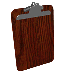
\includegraphics{images/report.pdf}}

\newcommand{\result}[1]{
\begin{verbatim}
	#1 
\end{verbatim}
} 
\newcommand{\prompt}[1]{#1:\textasciitilde\#}


%%%%%%%%%%%%%%%%%%%%%%%%%%%%%%%%%%%%%%
% exercise environment
%%%%%%%%%%%%%%%%%%%%%%%%%%%%%%%%%%%%%%

\newcounter{Exercisecount}[chapter]
\setcounter{Exercisecount}{0}
\newenvironment{exercise}[1]
{% This is the begin code
\refstepcounter{Exercisecount} {\textbf {Exercise \arabic{Exercisecount}}}: #1
}
{% This is the end code
 }

%%%%%%%%%%%%%%%%%%%%%%%%%%%%%%%%%%%%%%
% question counter environment
%%%%%%%%%%%%%%%%%%%%%%%%%%%%%%%%%%%%%%
\newcounter{questioncount}[Exercisecount]
\setcounter{questioncount}{0}

\newcommand{\answerlabel}{L\arabic{chapter}-\arabic{Exercisecount}-\arabic{questioncount}}

\newcommand{\answer}{
\begin{tikzpicture}
 
\node [fill=shade,rounded corners=5pt]
{
\refstepcounter{questioncount}
\color{white}{\textbf{\answerlabel}}
};
\end{tikzpicture}
}

\newcommand{\includeanswer}{\input{solutions/\answerlabel.tex}}


%%%%%%%%%%%%%%%%%%%%%%%%%%%%%%%%%%%%%%
% verbatim solution environment
%%%%%%%%%%%%%%%%%%%%%%%%%%%%%%%%%%%%%%
%\newcounter{linescounter}
%\newenvironment{esolution}[1]
%{
%\answer
%\ifthenelse{\boolean{Solutions}}
%{
%\color{blue}
%
%\hrulefill
%
%\includeanswer
%
%}
%{\setlength{\extrarowheight}{0.75cm} 
%
%\forloop{linescounter}{0}{\value{linescounter}<#1}{\quad\newline\vspace{12pt} \dotfill\newline}
%\comment
%}
%}

\newenvironment{esolution}
{
\answer
\ifthenelse{\boolean{Solutions}}
{
\color{blue}

\hrulefill

\includeanswer

}
{\setlength{\extrarowheight}{0.75cm} 
\quad\newline\vspace{12pt} \dotfill\newline
\comment
}
}
{
\ifthenelse{\boolean{Solutions}}
{

\hrulefill

}
{\endcomment}
}


\DefineVerbatimEnvironment{Verbatim}{Verbatim}
{formatcom=\color{blue},fontfamily=courier,fontseries=b,frame=lines,numbers=left}





%%%%%%%%%%%%%%%%%%%%%%%%%%%%%%%%%%%%%%
% shortcuts
%%%%%%%%%%%%%%%%%%%%%%%%%%%%%%%%%%%%%%
\newcommand{\wifi}{IEEE 802.11\xspace}

%%%%%%%%%%%%%%%%%%%%%%%%%%%%%%%%%%%%%%
% fonts
%%%%%%%%%%%%%%%%%%%%%%%%%%%%%%%%%%%%%%
\renewcommand{\rmdefault}{phv}
\renewcommand{\sfdefault}{phv}

%%%%%%%%%%%%%%%%%%%%%%%%%%%%%%%%%%%%%%
% colors
%%%%%%%%%%%%%%%%%%%%%%%%%%%%%%%%%%%%%%
\definecolor{shade}{HTML}{3877A9}	%light blue shade
\setlength{\parskip}{10pt plus 1pt minus 1pt}

\lstset{ %
basicstyle=\footnotesize,       % the size of the fonts that are used for the code
numbers=left,                   % where to put the line-numbers
numberstyle=\footnotesize,      % the size of the fonts that are used for the line-numbers
stepnumber=2,                   % the step between two line-numbers. If it's 1, each line 
                                % will be numbered
numbersep=5pt,                  % how far the line-numbers are from the code
backgroundcolor=\color{white},  % choose the background color. You must add \usepackage{color}
showspaces=false,               % show spaces adding particular underscores
showstringspaces=false,         % underline spaces within strings
showtabs=false,                 % show tabs within strings adding particular underscores
frame=single,                   % adds a frame around the code
tabsize=2,                      % sets default tabsize to 2 spaces
captionpos=b,                   % sets the caption-position to bottom
breaklines=true,                % sets automatic line breaking
breakatwhitespace=false,        % sets if automatic breaks should only happen at whitespace
title=\lstname,                 % show the filename of files included with \lstinputlisting;
                                % also try caption instead of title
escapeinside={\%*}{*)},         % if you want to add a comment within your code
morekeywords={*,...}            % if you want to add more keywords to the set
}